%%%%%%%%%%%%%%%%%%% vorlage.tex %%%%%%%%%%%%%%%%%%%%%%%%%%%%%
%
% LaTeX-Vorlage zur Erstellung von Projekt-Dokumentationen
% im Fachbereich Informatik der Hochschule Trier
%
% Basis: Vorlage svmono des Springer Verlags
%
%%%%%%%%%%%%%%%%%%%%%%%%%%%%%%%%%%%%%%%%%%%%%%%%%%%%%%%%%%%%%

\documentclass[envcountsame,envcountchap, deutsch]{i-studis}

\usepackage{makeidx}         	% Index
\usepackage{multicol}        	% Zweispaltiger Index
%\usepackage[bottom]{footmisc}	% Erzeugung von Fu�noten

%%-----------------------------------------------------
%\newif\ifpdf
%\ifx\pdfoutput\undefined
%\pdffalse
%\else
%\pdfoutput=1
%\pdftrue
%\fi
%%--------------------------------------------------------
%\ifpdf
\usepackage[pdftex]{graphicx}
\usepackage[pdftex,plainpages=false]{hyperref}
%\else
%\usepackage{graphicx}
%\usepackage[plainpages=false]{hyperref}
%\fi

%%-----------------------------------------------------
\usepackage{color}				% Farbverwaltung
%\usepackage{ngerman} 			% Neue deutsche Rechtsschreibung
\usepackage[english, ngerman]{babel}
\usepackage[latin1]{inputenc} 	% Erm�glicht Umlaute-Darstellung
%\usepackage[utf8]{inputenc}  	% Erm�glicht Umlaute-Darstellung unter Linux (je nach verwendetem Format)

%-----------------------------------------------------
\usepackage{listings} 			% Code-Darstellung
\lstset
{
	basicstyle=\scriptsize, 	% print whole listing small
	keywordstyle=\color{blue}\bfseries,
								% underlined bold black keywords
	identifierstyle=, 			% nothing happens
	commentstyle=\color{red}, 	% white comments
	stringstyle=\ttfamily, 		% typewriter type for strings
	showstringspaces=false, 	% no special string spaces
	framexleftmargin=7mm, 
	tabsize=3,
	showtabs=false,
	frame=single, 
	rulesepcolor=\color{blue},
	numbers=left,
	linewidth=146mm,
	xleftmargin=8mm
}
\usepackage{textcomp} 			% Celsius-Darstellung
\usepackage{amssymb,amsfonts,amstext,amsmath}	% Mathematische Symbole
\usepackage[german, ruled, vlined]{algorithm2e}
\usepackage[a4paper]{geometry} % Andere Formatierung
\usepackage{bibgerm}
\usepackage{array}
\hyphenation{Ele-men-tar-ob-jek-te  ab-ge-tas-tet Aus-wer-tung House-holder-Matrix Le-ast-Squa-res-Al-go-ri-th-men} 		% Weitere Silbentrennung bei Bedarf angeben
\setlength{\textheight}{1.1\textheight}
\pagestyle{myheadings} 			% Erzeugt selbstdefinierte Kopfzeile
\makeindex 						% Index-Erstellung


%--------------------------------------------------------------------------
\begin{document}
%------------------------- Titelblatt -------------------------------------
\title{B-Baum-Datenstruktur}
\project{Ausarbeitung zur Vorlesung Wissenschaftliches Arbeiten}
%--------------------------------------------------------------------------
\supervisor{Titel Vorname Name} 		% Betreuer der Arbeit
\author{Bearbeiter 1: Sharif El Deib \\Bearbeiter 2: Dominik Petersdorf \\Bearbeiter 3: Carlos De Sa e Matos}							% Autor der Arbeit
\groupid{48}
\address{Ort,} 							% Im Zusammenhang mit dem Datum wird hinter dem Ort ein Komma angegeben
\submitdate{Abgabedatum} 				% Abgabedatum
%\begingroup
%  \renewcommand{\thepage}{title}
%  \mytitlepage
%  \newpage
%\endgroup
\begingroup
  \renewcommand{\thepage}{Titel}
  \mytitlepage
  \newpage
\endgroup
%--------------------------------------------------------------------------
\frontmatter 
%--------------------------------------------------------------------------
%\kurzfassung

%% deutsch
\paragraph*{}
In der Kurzfassung soll in kurzer und pr�gnanter Weise der wesentliche Inhalt der Arbeit beschrieben werden. Dazu z�hlen vor allem eine kurze Aufgabenbeschreibung, der L�sungsansatz sowie die wesentlichen Ergebnisse der Arbeit. Ein h�ufiger Fehler f�r die Kurzfassung ist, dass lediglich die Aufgabenbeschreibung (d.h. das Problem) in Kurzform vorgelegt wird. Die Kurzfassung soll aber die gesamte Arbeit widerspiegeln. Deshalb sind vor allem die erzielten Ergebnisse darzustellen. Die Kurzfassung soll etwa eine halbe bis ganze DIN-A4-Seite umfassen.

Hinweis: Schreiben Sie die Kurzfassung am Ende der Arbeit, denn eventuell ist Ihnen beim Schreiben erst vollends klar geworden, was das Wesentliche der Arbeit ist bzw. welche Schwerpunkte Sie bei der Arbeit gesetzt haben. Andernfalls laufen Sie Gefahr, dass die Kurzfassung nicht zum Rest der Arbeit passt.

%% englisch
\paragraph*{}
The same in english.
 			% Kurzfassung Deutsch/English
\tableofcontents 						% Inhaltsverzeichnis
%--------------------------------------------------------------------------
\mainmatter                        		% Hauptteil (ab hier arab. Seitenzahlen)
%--------------------------------------------------------------------------
% Die Kapitel werden in separaten .tex-Dateien abgelegt und hier eingebunden.
%Unsere Arbeit
\chapter{Einleitung}
\begin{flushleft}	
Die Aufgabe von Datenbanken ist die Verwaltung von gro�en Datenmengen. D.h. man
will verschiedene Operationen auf diesen Daten m�glichst schnell ausf�hren k�nnen.
Man muss die Informationen also in einer Datenstruktur abspeichern, die die
entsprechenden Operationen in einer m�glichst effizienten Weise unterst�tzen.
Man muss sich also die Frage stellen, welche Datenstruktur hierf�r geeignet ist und warum?
B-B�ume wurden von Prof. Rudolf Bayer explizit f�r die Plattenspeicherverwaltung
entworfen. F�r seine Arbeiten rund um den B-Baum und andere Verdienste erhielt Prof. 
Rudolf Bayer im Jahr (2001) den \glqq SIGMOD Innovations award\grqq. In unserer Arbeit setzen wir uns unter anderem mit dem Grund auseinander, warum B-B\"aume f�r die Plattenspeicherverwaltung geeignet ist. Dabei ist es zwangsweise notwendig die B-B\"aume genauer zu betrachten, und die in dieser Arbeit behandelten Themen n\"aher zu behandeln.
Zun�chst werden wir die B-B\"aume genauer definieren, gefolgt von der Behandlung der Operationen in B-B\"aumen. Anschlie\ss end werden noch die Komplexit\"atsklassen angesprochen und eine genauere Beschreibung der Anwendungen.
\end{flushleft}
\chapter{Definition B-Baum}

Ein B-Baum ist ein balancierter Suchbaum der Ordnung $n$, wenn es folgende Eigenschaften enth\"alt:

	\begin{enumerate}
		\item Jeder Knoten besitzt mindestens $1$ und h\"ochstens $n-1$ Elemente.
		\item Jeder Knoten mit $m$ Elemente hat $m+1$ S\"ohne, au\ss er Bl\"atter.
		\item Jeder Wert der Elemente im linken Teil des Baumes ist kleiner als die Werte des rechten Teil des Baumes.
		\item Alle Bl\"atter m\"ussen die gleiche Tiefe $h$ haben und d\"urfen keinen Nachfolger geben.
	\end{enumerate}
Nehmen wir einen B-Baum der Ordnung $3$ als Beispiel(siehe Abb. \ref{d1}). Jeder Knoten dieses Baumes kann zwischen 1 und 3 Elemente haben. Ein innere Knoten hat im unseren Beispiel 3 S\"ohne. Die Werten der Elemente erh\"ohen sich vom linken Teil bis zum rechten Teil des Baumes. Dazu kommt noch, dass jedes Blatt die gleiche Tiefe hat. Im diesen Fall hat jedes Blatt die Tiefe $3$.
Somit stimmen alle oben genannten Eigenschaften \"uberein.
\begin{figure}[h!] %[hbtp]
	\centering
		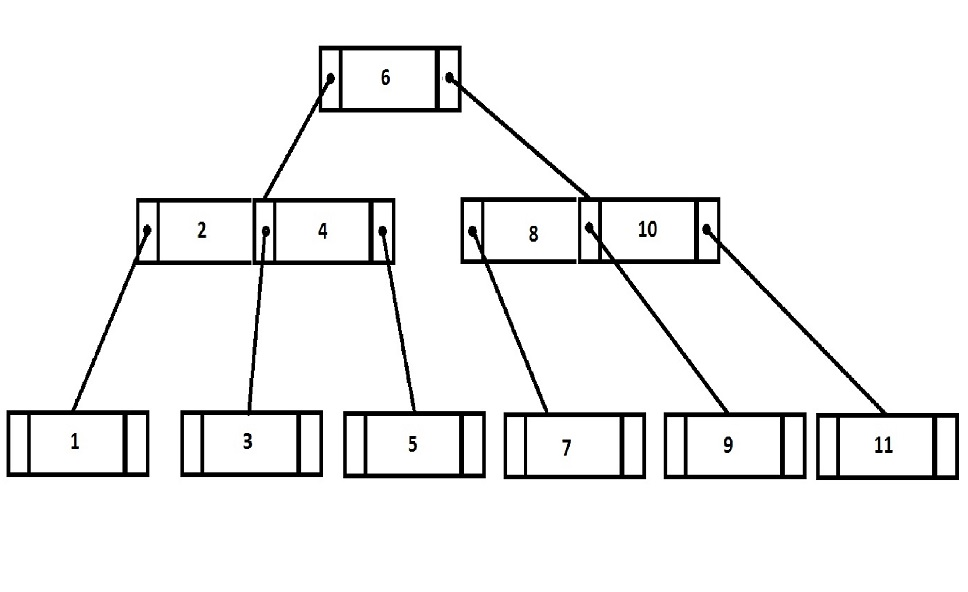
\includegraphics[scale=0.5]{images/definition.jpg}
	\caption{Beispiel eines B-Baumes}
	\label{d1}
\end{figure}

\paragraph{}
Es gibt ein spezieller B-Baum, der $1$,$2$ oder $3$ Elemente pro Knoten hat und $2$, $3$ oder $4$ S\"ohne haben kann. Dieser Baum wird als 2-3-4-Baum gekennzeichnet(siehe Abb. \ref{b234}).
\begin{figure}[h!] %[hbtp]
	\centering
		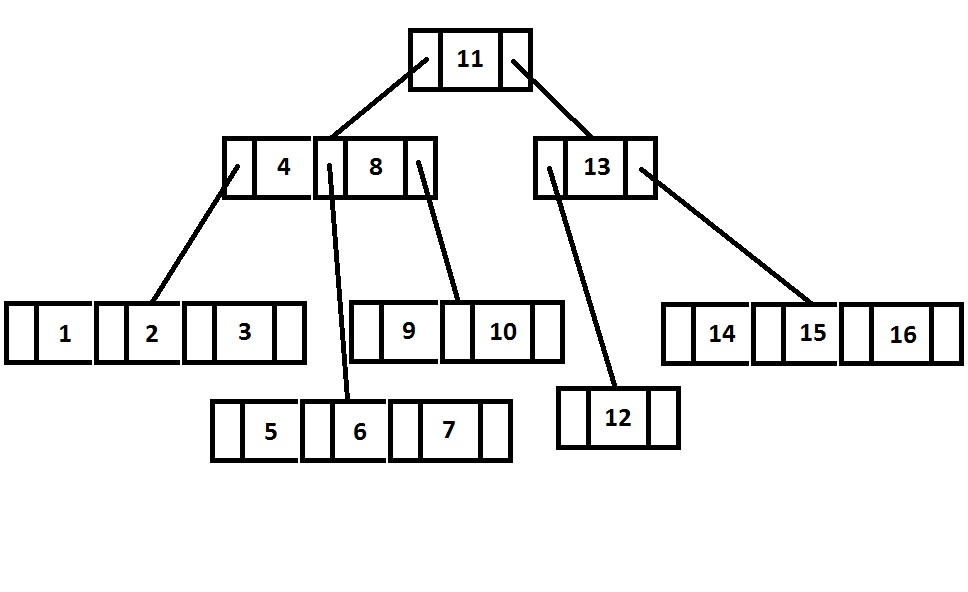
\includegraphics[scale=0.5]{images/234baum.jpg}
	\caption{2-3-4-Baum}
	\label{b234}
\end{figure}
\chapter{Operationen}

\section{Suchen}

Um einen Schl\"ussel innerhalb eines B-Baums zu suchen geht man folgenderma\ss en vor. Ausgehend von der Wurzel werden alle Knoten danach \"uberpr\"uft, ob sich der Schl\"ussel in dem betrachteten Knoten befindet. Wird er nicht in der Wurzel gefunden wird der kleinste Schl\"ussel, der gr\"o\ss er als der gesuchte Schl\"ussel ist bestimmt. Sofern dieser Schl\"ussel existiert, wird bei dem Kindknoten links von diesem weitergesucht. Wenn die Suche am Ende bei einer null-Referenz landet existiert der Schl\"ussel nicht, oder er wurde nicht gefunden. 
\\[0.5in]
\begin{figure}[h!] %[hbtp]
	\centering
	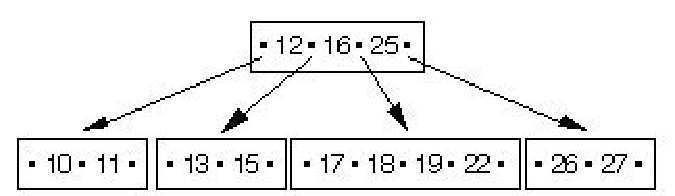
\includegraphics[width=0.7\linewidth]{images/Beispiel_Suche_B-Baum.pdf}
	\caption{Beispiel B-Baum}
	\label{Beispiel_Suche_B-Baum}
\end{figure}
\\[0.3in]
\section{Einf\"ugen}
Damit ein neuer Knoten eingef\"ugt werden kann, wird zuerst das Blatt bestimmt in dem sich der Schl\"ussel befinden m\"usste. Daher es den Schl\"ussel noch nicht gibt, bleibt die Suche erfolglos. Nun k\"onnen 2 F\"alle eintreten, wie der neue Schl\"ussel in den B-Baum eingef\"ugt werden kann. Hierbei ist zu beachten, dass nur $m-1$ Schl\"ussel pro Knoten gespeichert werden k\"onnen. 
\paragraph{Fall 1.}
Der Knoten k hat m-1 Schl\"ussel noch nicht gespeichert und es wurde der Schl\"ussel $x$ auch in der Blattebene nicht gefunden, so wird der Schl\"ussel in den B-Baum eingef\"ugt. In diesem Fall f\"ugt man den Schl\"ussel $x$ in dem Knoten $k$ zwischen $x_{i}$ und $ x_{i+1} $ ein.
\newline
Ein Beispiel:
\newline
Wir f\"ugen in (siehe Abb. \ref{Beispiel_Suche_B-Baum})  den Schl\"ussel 14 ein. Zuerst beginnt der Suchbaum in der Wurzel $-12-16-$($12<14>16$), der Schl\"ussel wechselt in den Kindknoten zwischen 12 und 16. Dieser Knoten besitzt die Schl\"ussel $-13-15-$. Daher der B-Baum die Ordnung $m=5$ besitzt, ist in dem Knoten noch Platz f\"ur einen weiteren Schl\"ussel. Dort wird der Schl\"ussel nach der Definition (siehe Kapitel \ref{def}) eingef\"ugt.(siehe Abb. \ref{insert_01}) 
\\[0.5in]
\begin{figure}[h!] %[hbtp]	
\centering
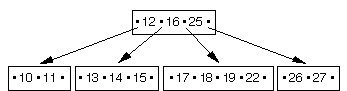
\includegraphics[width=0.7\linewidth]{images/insert_01}
\caption{14 einf\"ugen}
\label{insert_01}
\end{figure}
\\[0.3in]
\paragraph{Fall 2:}
Es wurden bereits $m-1$ Schl\"ussel in dem Knoten gespeichert, zudem der Schl\"ussel $x$ geh\"oren w\"urde. Der Schl\"ussel wird daher zuerst in den betreffenden Knoten seiner Gr\"o\ss e nach eingef\"ugt und der zu gro\ss e Knoten in der Mitte geteilt. Der mittlere Knoten wandert in seinen Vaterknoten und ordnet sich dort seiner Gr\"o\ss e nach ein. Die Zeiger auf die Kindknoten passen sich der neuen Anordnung an.
\newline
Ein Beispiel:
\newline
In die vorherige Abbildung (siehe Abb. \ref{insert_01}) wird der neue Schl\"ussel $24$ eingef\"ugt. Daher der Knoten zu gro\ss  wird, teilt er sich und der Schl\"ussel $19$ wandert in den Vaterknoten. Danach bilden sich 2 neue Knoten aus dem zu gross{}en Knoten.(siehe Abb. \ref{insert_02})
\\[0.5in]
\begin{figure}[h!] %[hbtp]	
	\centering
	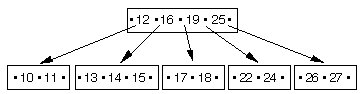
\includegraphics[width=0.7\linewidth]{images/insert_02}
	\caption{24 einf\"ugen}
	\label{insert_02}
\end{figure}
\newpage
\section{L\"oschen}
L\"oschen in B-B\"aumen ist im Gegenzug zu anderen B\"aumen komplexer, da sehr genau zwischen dem L\"oschen von Knoten und von Bl\"attern unterschieden werden muss.
Hierbei kann man 3 F\"alle unterscheiden.
\begin{enumerate}
	\item Wenn das Blatt die Wurzel ist und das Blatt leer ist kann die Wurzel gel\"oscht werden. Der Baum ist leer.
	\item Wenn das Blatt nicht die Wurzel ist, und  $m\geq \lceil n/2\rceil-1$ Schl\"ussel besitzt. Dann ist das L\"oschen beendet.
	\item Wenn jedoch $m= \lceil n/2\rceil-2$, so muss die Eigenschaft des B-Baums wiederhergestellt werden.
		\begin{enumerate}
				\item Gibt es einen Nachbarn, der $m> \lceil n/2\rceil-1$, so k\"onnen Schl\"ussel zwischen den beiden Knoten verschoben werden.
				\item Gilt f\"ur beide Knoten jedoch, $m= \lceil n/2\rceil-1$, so m\"ussen 2 Knoten vereinigt werden.
		\end{enumerate}	
\end{enumerate}

\paragraph{Verschiebung von Schl\"usseln beim L\"oschen} 
\begin{tabular}{|l|l|}
	\hline \\Nur rechter Nachbar vorhanden mit\\ $m_{rechts}> \lceil n/2\rceil -1$  & Linksverschiebung  \\ 
	\hline \\Linker und rechter Nachbar vorhanden mit\\ $m_{links>}> \lceil n/2\rceil -1$ und $m_{rechts>}> \lceil n/2\rceil -1$ und $ m_{links} m_{rechts}$ & Linksverschiebung \\ 
	\hline \\Linker und rechter Nachbar vorhanden mit\\ $m_{links>}> \lceil n/2\rceil -1$ und $m_{rechts>}> \lceil n/2\rceil -1$ und $ m_{links} m_{rechts}$ & Rechtsverschiebung \\ 
	\hline \\nur linker Nachbar vorhanden mit\\ $m_{rechts}> \lceil n/2\rceil -1$ & Rechtsverschiebung \\ 
	\hline 
\end{tabular} 
([Schroeder:03], S. 5)
\newpage
\paragraph{Vereinigung von Knoten beim L\"oschen} 

Vereinigung mit rechtem Nachbarn nach L\"oschen von a3(siehe Abb. \ref{loeschen_01})
\begin{figure}[h!] %[hbtp]	
	\centering
	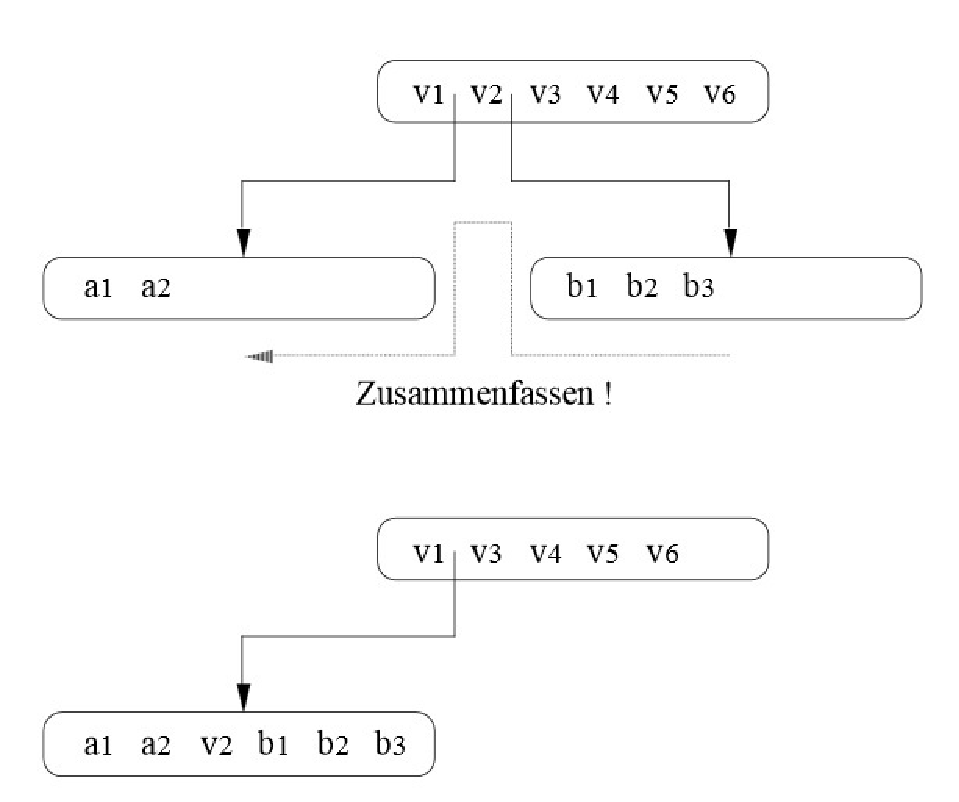
\includegraphics[width=0.7\linewidth]{images/loeschen_01}
	\caption{([Schroeder:03], S. 6)}
	\label{loeschen_01}
\end{figure}
\begin{itemize}
	\item Durch das Vereinigen von Knoten wird die Zahl der Werte m im Vorg\"angerknoten um eins kleiner.
	\item Daher kann dort wiederum ein Unterschreiten der Untergrenze stattfinden.
	\item Vereinigungsvorg\"ange k\"onnen sich daher bis zur Wurzel fortsetzen.
	\item ie Wurzel selbst darf jedoch weniger als $\lceil n/2\rceil -1$ Werte besitzen, so dass hier der Vorgang endet
	
\end{itemize}
\chapter{Komplexit�t}

Wir wollen hier die Zeitkomplexit�t zum Durchlaufen und Finden eines bestimmten Datenelementes in einem B Baumes untersuchen. Diese gibt an, wovon der Zeitaufwand abh�ngt, um den B Baum nach einem Datenelement zu durchsuchen. Sowohl die der Zeitaufwand der  Operationen  Finden, Einf�gen und L�schen h�ngen auch direkt von diesem Zeitaufwand ab.  So wie logischerweise  zum L�schen eines Datenelementes dieses vor der eigentlichen Operation zuerst gefunden werden muss, muss auch vor dem Einf�gen zuerst festgestellt werden an welche Stelle das neue Element eingef�gt werden muss, damit die Ordnung der Datenelemente immer noch gew�hrleistet ist. Diese Ortung der Einf�gstelle kommt einem Finden (zum Beispiel des Nachbarelementes) gleich.
Bei der exakten Betrachtung von Laufzeiten, m�ssten viele verschiedene F�lle unterschieden werden, so wird sich oft darauf beschr�nkt die Komplexit�tsklasse des Laufzeitverhaltens zu bestimmen, d. h. es wird bestimmt welcher Klasse von Funktionen die Laufzeitfunktion geh�rt (linear, quadratisch, logarithmisch...). Die sogenannte Komplexit�tsklasse ist im Vergleich zur genauen Laufzeitfunktion einfacher zu bestimmen. Zwar ist eine genaue Berechnung der eigentlichen Laufzeit nicht m�glich, aber es ist m�glich eine asymptotische Obergrenze der Laufzeit und einen Vergleich zwischen verschiedenen Strukturen und Algorithmen zu erstellen. 


\section{Komplexit�tsklasse beim B-Baum}

Zun�chst m�ssen wir uns mit der Struktur des B Baumes befassen, um eine Komplexit�tsklasse der Operationen auf den B Baum bestimmen zu k�nnen. Hierzu zuerst einige Definitionen und Notationen:
Man nennt Tiefe t, den Abstand eines beliebigen Knotens zur Wurzel.
Man nennt H�he h eines B Baumes den Abstand von der Wurzel zu den Bl�ttern, es ist also die Tiefe t der Bl�tter.
Die Wurzel ist der Vorfahre jedes Knotens.
Ein Blatt ist ein Feld mit Datenelementen und befindet sich am ?Ende? des Baumes, d. H. ein Blatt hat keine Nachkommen (S�hne). 
Eine spezielle Eigenschaft des B Baumes ist es, dass alle Bl�tter die gleiche Tiefe T besitzen und stellen somit die H�he h des B Baumes dar.
Um ein Datenelement zu finden, das sich gezwungenerweise in den Bl�ttern befindet, muss ein Algorithmus die Datenstruktur von der Wurzel bis zu dem gesuchten Blatt durchlaufen, also die H�he h durchlaufen. Auf dem Weg von einem Knoten zum anderen, muss es einen Speicherzugriff geben, die Anzahl der Speicherzugriffe von der Wurzel zum Blatt ist immer gleich der H�he h. Folglich ist die Komplexit�t der meisten Operationen (Find, Insert , Delete) auf B B�umen proportional zur H�he h des B Baumes.

Wir wollen nun die H�he h des B Baumes in Zusammenhang mit der gesamten Anzahl \# von Datenelementen im B Baum bringen. Dazu m�ssen wir entscheiden wie viele Kinder jeder Knoten haben soll, sei 2n diese maximale Anzahl der Kinder. Je nach dem F�llgrad der Knoten, der bei einem B Baum f�r jeden Knoten zwischen mindestens n und maximal 2n liegt, ergeben sich verschiedene H�hen f�r die gleiche Anzahl von Datenelementen ?. Die gr�\ss te H�he h, d.h. die l�ngste Laufzeit, weist ein B Baum auf, falls jeder Knoten nur die H�lfte der m�glichen Kinder aufweist. Dagegen hat ein B Baum mit ? Datenelementen die k�rzeste H�he h, und somit auch die k�rzeste Laufzeit, falls jeder Knoten die maximal m�gliche Anzahl von Kindern d. h. 2n aufweist. Daher ergeben sich folgende Grenzwerte f�r h :
\\[0.5in]
{\large \centerline {$\log_2n+1 {(\#+1)-1} \leq h \leq  \log_n+1 {(\frac{\#+1}{2})}$} }


\chapter{Anwendung von B-B\"aume}

Heutzutage werden die B-B\"aume in Datenbanksystemen benutzt, die sehr hohe Datenmengen haben. Diese Datenstruktur verk\"urzt die Zeit die es ben\"otigt, um eine gew\"ahlte Menge von Daten zu suchen. Haupts\"achlich wird der B-Baum in Luft- und Raumfahrtindustrie eingesetzt.

\paragraph{}
Ein gutes Beispiel ist ein PC den man zu Hause stehen hat. Ein PC besitzt ein Hauptspeicher und eine Festplatte. Da der Hauptspeicher eine schnellen Lese/Schreiben-Zugriff haben muss, k\"onnte man unm\"oglich die ganzen Datenmengen in dem Hauptspeicher speichern. Denn dies wurde den Zugriff verlangsamen. Deshalb werden im Hauptspeicher lediglich die Werte der Schl\"ussel gespeichert und die gro\ss en Datenmengen werden auf der Festplatte gespeichert. Die Schl\"ussel haben die Verweise auf die Sektorbl\"ocke der Festplatte. Dies erh\"oht die Lese- und Schreibgeschwindigkeit, denn die Zugriff maximiert sich auf die Tiefe des Baumes.
% ...
%--------------------------------------------------------------------------
\backmatter                        		% Anhang
%-------------------------------------------------------------------------
\bibliographystyle{geralpha}			% Literaturverzeichnis
\bibliography{literatur}     			% BibTeX-File literatur.bib
%--------------------------------------------------------------------------
\printindex 							% Index (optional)
%--------------------------------------------------------------------------
\begin{appendix}						% Anh�nge sind i.d.R. optional
   %\chapter{Glossar}

\abbreviation{DisASTer}		{DisASTer (Distributed Algorithms Simulation Terrain), A platform for the Implementation of Distributed Algorithms}
\abbreviation{DSM}			{Distributed Shared Memory}
\abbreviation{AC}			{Linearisierbarkeit (atomic consistency)}
\abbreviation{SC}			{Sequentielle Konsistenz (sequential consistency)}
\abbreviation{WC}			{Schwache Konsistenz (weak consistency)}
\abbreviation{RC}			{Freigabekonsistenz (release consistency)}
			% Glossar   
\end{appendix}

\end{document}
